\documentclass[11pt]{article}

%% MinionPro fonts 
%\usepackage[lf]{MinionPro}
%\usepackage{MnSymbol}
\usepackage{microtype}

%% Margins
\usepackage{geometry}
\geometry{verbose,letterpaper,tmargin=1in,bmargin=1in,lmargin=1in,rmargin=1in}

%% Other packages
\usepackage{amsmath}
\usepackage{amsthm}
\usepackage[shortlabels]{enumitem}
\usepackage{titlesec}
\usepackage{soul}
\usepackage{tikz}
\usepackage{mathtools}
\usepackage{pgfplots}
\usepackage{tikz-3dplot}
\usepackage{algorithmic}
\usepackage[export]{adjustbox}
\usepackage{tcolorbox}
\usepackage{mathrsfs}

%% Paragraph style settings
\setlength{\parskip}{\medskipamount}
\setlength{\parindent}{0pt}

%% Change itemize bullets
\renewcommand{\labelitemi}{$\bullet$}
\renewcommand{\labelitemii}{$\circ$}
\renewcommand{\labelitemiii}{$\diamond$}
\renewcommand{\labelitemiv}{$\cdot$}

%% Colors
\definecolor{rred}{RGB}{204,0,0}
\definecolor{ggreen}{RGB}{0,145,0}
\definecolor{yyellow}{RGB}{255,185,0}
\definecolor{bblue}{rgb}{0.2,0.2,0.7}
\definecolor{ggray}{RGB}{190,190,190}
\definecolor{ppurple}{RGB}{160,32,240}
\definecolor{oorange}{RGB}{255,165,0}

%% Shrink section fonts
\titleformat*{\section}{\normalsize\bf}
\titleformat*{\subsection}{\normalsize\bf}
\titleformat*{\subsubsection}{\normalsize\it}

% %% Compress the spacing around section titles
\titlespacing*{\section}{0pt}{1.5ex}{0.75ex}
\titlespacing*{\subsection}{0pt}{1ex}{0.5ex}
\titlespacing*{\subsubsection}{0pt}{1ex}{0.5ex}

%% amsthm settings
\theoremstyle{definition}
\newtheorem{problem}{Problem}
\newtheorem{example}{Example}
\newtheorem*{theorem}{Theorem}
\newtheorem*{bigthm}{Big Theorem}
\newtheorem*{biggerthm}{Bigger Theorem}
\newtheorem*{bigcor1}{Big Corollary 1}
\newtheorem*{bigcor2}{Big Corollary 2}

%% tikz settings
\usetikzlibrary{calc}
\usetikzlibrary{patterns}
\usetikzlibrary{decorations}
\usepgfplotslibrary{polar}

%% algorithmic setup
\algsetup{linenodelimiter=}
\renewcommand{\algorithmiccomment}[1]{\quad// #1}
\renewcommand{\algorithmicrequire}{\emph{Input:}}
\renewcommand{\algorithmicensure}{\emph{Output:}}

%% Answer box macros
%% \answerbox{alignment}{width}{height}
\newcommand{\answerbox}[3]{%
  \fbox{%
    \begin{minipage}[#1]{#2}
      \hfill\vspace{#3}
    \end{minipage}
  }
}

%% \answerboxfull{alignment}{height}
\newcommand{\answerboxfull}[2]{%
  \answerbox{#1}{6.38in}{#2} 
}

%% \answerboxone{alignment}{height} -- for first-level bullet
\newcommand{\answerboxone}[2]{%
  \answerbox{#1}{6.0in}{#2} 
}

%% \answerboxtwo{alignment}{height} -- for second-level bullet
\newcommand{\answerboxtwo}[2]{%
  \answerbox{#1}{5.8in}{#2}
}

%% special boxes
\newcommand{\wordbox}{\answerbox{c}{1.2in}{.7cm}}
\newcommand{\catbox}{\answerbox{c}{.5in}{.7cm}}
\newcommand{\letterbox}{\answerbox{c}{.7cm}{.7cm}}

%% Miscellaneous macros
\newcommand{\tstack}[1]{\begin{multlined}[t] #1 \end{multlined}}
\newcommand{\cstack}[1]{\begin{multlined}[c] #1 \end{multlined}}
\newcommand{\ccite}[1]{\only<presentation>{{\scriptsize\color{gray} #1}}\only<article>{{\small [#1]}}}
\newcommand{\grad}{\nabla}
\newcommand{\ra}{\ensuremath{\rightarrow}~}
\newcommand{\maximize}{\text{maximize}}
\newcommand{\minimize}{\text{minimize}}
\newcommand{\subjectto}{\text{subject to}}
\newcommand{\trans}{\mathsf{T}}
\newcommand{\bb}{\mathbf{b}}
\newcommand{\bx}{\mathbf{x}}
\newcommand{\bc}{\mathbf{c}}
\newcommand{\bd}{\mathbf{d}}

%% LP format
%    \begin{align*}
%      \maximize \quad & \mathbf{c}^{\trans} \mathbf{x}\\
%      \subjectto \quad & A \mathbf{x} = \mathbf{b}\\
%                       & \mathbf{x} \ge \mathbf{0}
%    \end{align*}


%% Redefine maketitle
\makeatletter
\renewcommand{\maketitle}{
  \noindent SA405 -- AMP \hfill Rader \S 3.4--Page 103 \\

  \begin{center}\Large{\textbf{\@title}}\end{center}
}
\makeatother

%% ----- Begin document ----- %%
\begin{document}
  
\title{Lesson 11.  Traveling Salesperson Problem (TSP)}

\maketitle

%%%
\section{Tours and TSP}

\begin{tcolorbox}
A \textbf{tour} is a closed route that visits every location exactly once.

\smallskip
In graph terminology, a \textbf{tour} is a single cycle (collection of edges) that visits each node exactly once. This is also known as a Hamiltonian Cycle or Hamiltonian Circuit.
\end{tcolorbox}

\begin{problem}
For each graph below, does the set of edges represent a tour through the 6 nodes?  If not, explain why not.

\begin{center}
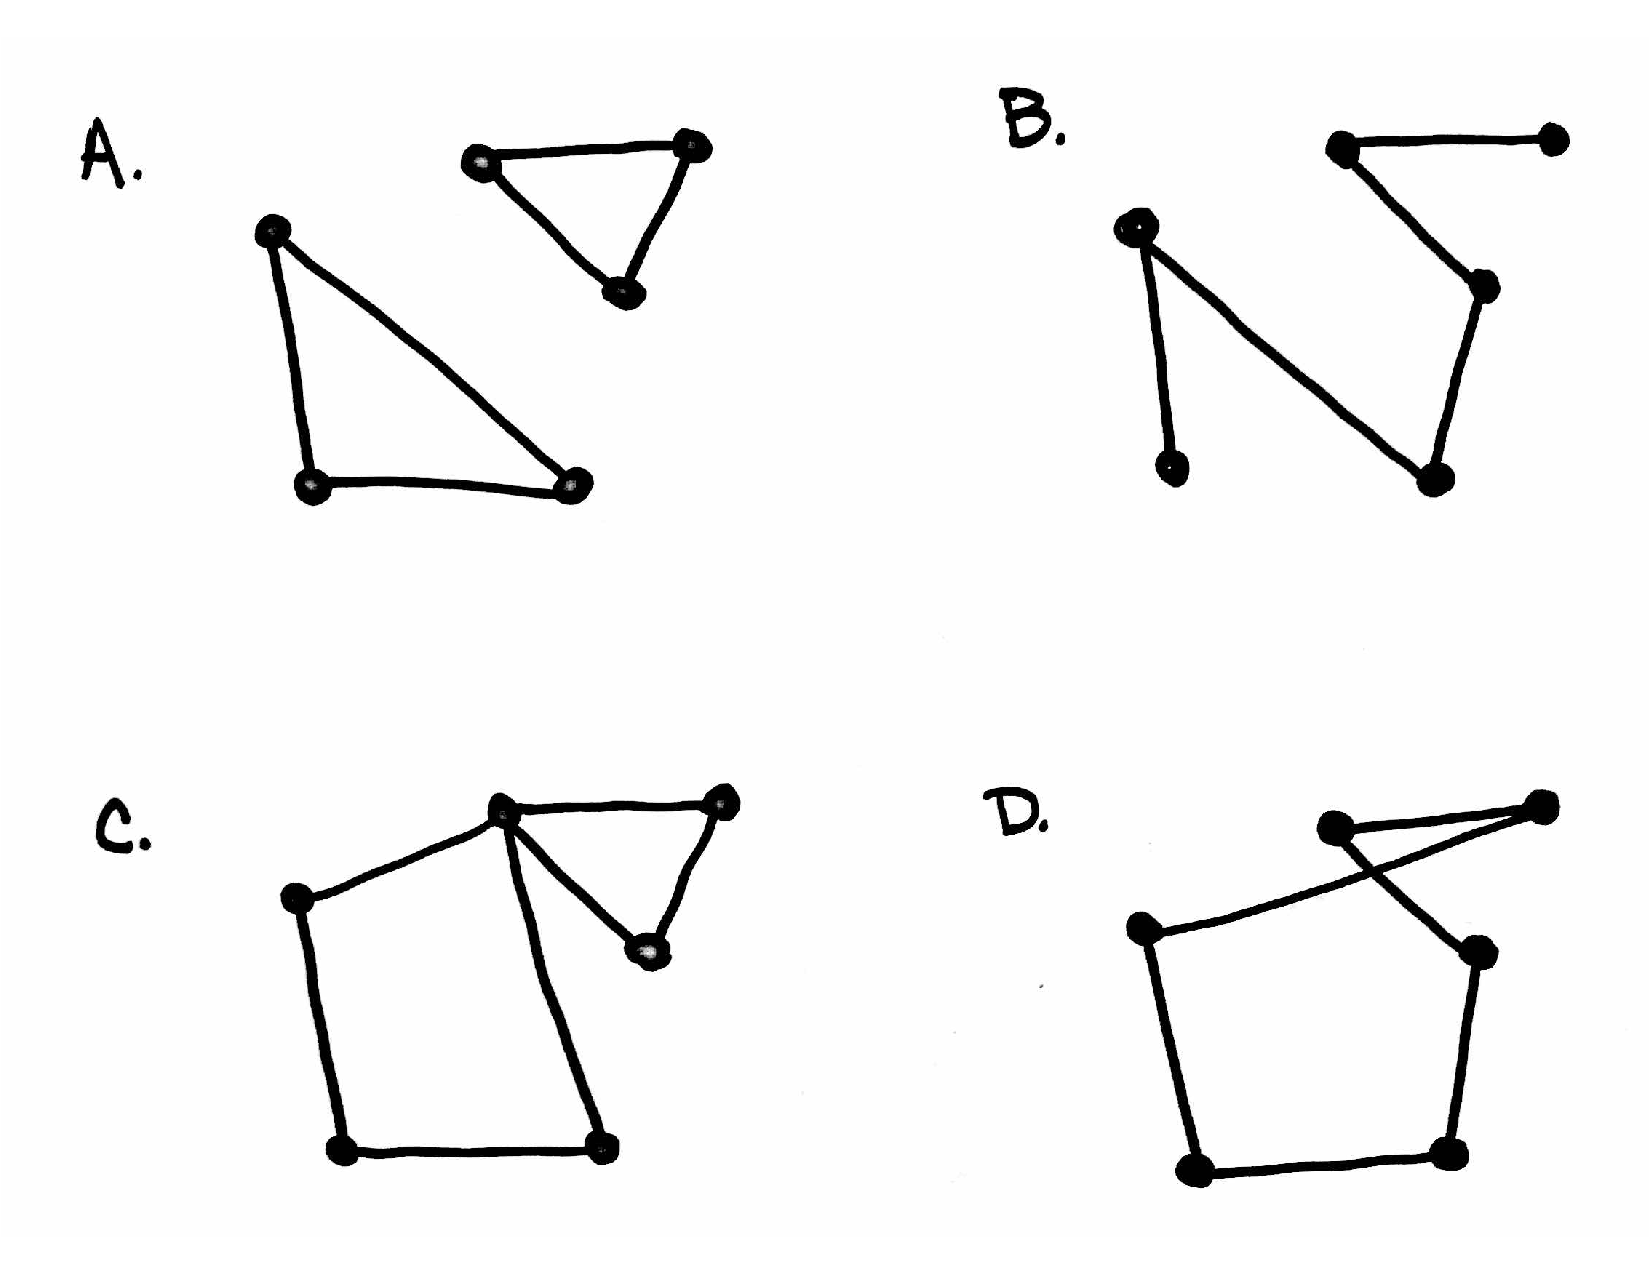
\includegraphics[width=0.6\textwidth]{tours}
\end{center}
\end{problem}

\begin{tcolorbox}
Given a graph $G = (V, E)$ with edge weights (representing costs or distances), the \textbf{Traveling Salesperson Problem (TSP)} seeks a \emph{minimum cost tour of} $G$.
\end{tcolorbox}

\begin{enumerate}
\item If we were to formulate this problem like the MST problem, what would be the decisions (in words) for the integer programming formulation?
\end{enumerate}

\newpage

\section{History of the TSP}

\begin{itemize}
\item TSP was first studied in the 1930s! The first IP formulation of TSP (which we're studying mostly in these notes) was in 1954.
\item Nowadays TSP has been solved on graphs with as many as 50,000 nodes such as a historic tour of the US.
\end{itemize}

\section{Visiting Graduate Schools: IP Formulation of TSP}

\begin{problem}
A college student is interested in visiting as many graduate schools as possible.
She reasons that a single visit to each school is appropriate, and she wants to 
return to her own campus only after visiting all the schools.  It is conceivable that
she visits the schools in any order, but she would like to minimize the amount of
driving she has to do.  If the distance between schools $i$ and $j$ is $d_{i,j}$ ($i < j$), where the 
matrix $D$ of distances is given below, in which order should she visit the schools?
Note that school 1 is her current school.

\[
D = \left[
\begin{array}{c|ccccc}
& 2 & 3 & 4 & 5 & 6 \\
\hline
1 & 16 & 23 & 14 & 8 & 15 \\
2 & - & 12 & 19 & 9 & 13 \\
3 & - & - & 7 & 25 & 16 \\
4 & - & - & - & 18 & 15 \\
5 & - & - & - & - & 20 \\
\end{array}
\right]
\]

\begin{enumerate}[resume]
\item Draw the graph $G = (V,E)$ of the network below.  Include node labels and edge costs.  Highlight a collection of edges that form a tour of the graph (doesn't have to be the minimum distance tour).

\vfill


\item Define the Sets, Variables, and Parameters that are needed for the IP model. 
\vfill \newpage


\item Write the objective function for this model. \vspace{1.25in}

\item There are two types of constraints that should be included in this model:
	\begin{enumerate}
	\item A cycle on $n$ nodes has exactly \catbox edges
	\item In order to have a tour, each node must be connected to exactly \catbox edges.
	\end{enumerate}
Write each of these constraints in both concrete/parameterized form.



\newpage
\item Is there a solution for this graph that satisfies these two constraints but is not a tour? \emph{Think back to MST.}

\vspace{2.5in}


\item Write concrete constraint(s) that prevents the graph that you sketched above from being selected by the solver.  \vspace{1.25in}



\item Write a parameterized constraint which prevents ANY graphs of this kind from being returned by the solver. Recall that there is one such constraint for every subset $S$ of vertices in $V$ such that \wordbox (restrict the number of vertices in $S$). These are called \textbf{subtour elimination constraints}.
\vfill
\newpage

\end{enumerate}

\end{problem}

\newpage

\section{Another Formulation of TSP}

The formulation we saw here is a so-called edge based TSP formulation and dates back to 1954. Recall the major drawback was that there are an exponential number of subtour elimination constraints.

Another possible formulation, which dates to the 2000s, has an exponential number of variables. Here we will discuss it.

\begin{enumerate}
\item Define a set $T$ which is the set of all possible tours of $N$.
	\begin{itemize}
	\item If $N$ has 4 nodes, how many possible tours/cycles are there? \vspace{2in}
	\item For a general graph with $n$ nodes, how many possible tours/cycles are there? \vspace{1in}
	\end{itemize}
\item Define a variable $x_i$ for all $i \in T$. $x_i = 1$ if tour $i$ is chosen and 0 otherwise. \vspace{1in}
\item Let $c_i$ be the cost of tour $i$ for all $i \in T$. \newpage
\item Using the sets $N, E,$ and $T$, and the variables/parameters $x_i$, $c_i$ for all $i \in T$; write a parameterized formulation for the TSP problem that has an exponential number of variables. \
\end{enumerate}

\vfill
\begin{tcolorbox}
Formulations like this can be more effective than the edge based formulations depending on the application area; however implementing them can be quite difficult. You can learn about how to solve a problem like this in either an advanced OR course and/or a capstone/honors project. 
\end{tcolorbox}

\end{document}

